\documentclass[tikz, 14pt, border=10pt]{standalone}
\usepackage[utf8]{inputenc}
\usepackage{amsmath}
\usepackage{amsfonts}
\usepackage{amssymb}
\usepackage{amsthm}
\usepackage{natbib}
\usepackage{geometry}
\usepackage{tikz}
\usepackage{textcomp}
\usepackage{multirow}
\usepackage{listings}
\usepackage[utf8]{inputenc}
\usepackage[english]{babel}
\usepackage{accents}
\usepackage{hyperref}
\usepackage[T1]{fontenc}
\usepackage{accents}
\newcommand{\ubar}[1]{\underaccent{\bar}{#1}}
\usetikzlibrary{shapes, snakes, patterns, arrows}
\geometry{portrait, margin=1in}
\linespread{1.2}
\setlength\parindent{0pt}

\begin{document}
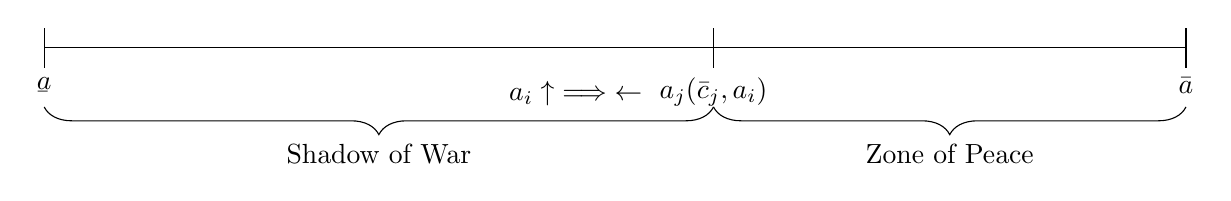
\begin{tikzpicture}
\draw (0.5,0) -- (15,0);
\draw (0.5,0.25) -- (0.5, -0.25) node[below] {$\ubar{a}$};
\draw (7.25, -0.3) node[below] {$a_i \uparrow \implies \leftarrow$};
\draw (9,0.25) -- (9, -0.25) node[below] {$a_j(\bar{c}_j, a_i)$};
\draw (15,0.25) -- (15, -0.25) node[below] {$\bar{a}$};
\draw [decorate,decoration={brace,amplitude=10pt,mirror}](0.5,-.75) -- (9,-.75) node[black,midway,yshift=-0.6cm] {\text{Shadow of War}};
\draw [decorate,decoration={brace,amplitude=10pt,mirror}](9,-.75) -- (15,-.75) node[black,midway,yshift=-0.6cm] {\text{Zone of Peace}};
\end{tikzpicture}
\end{document}